\documentclass[11pt,paper=a4,answers, addpoints]{exam}
\usepackage{graphicx,lastpage}
\usepackage{upgreek}
\usepackage{censor}
\censorruledepth=-.2ex
\censorruleheight=.1ex
\hyphenpenalty 10000

\usepackage[paperheight=10.5in,paperwidth=8.27in,bindingoffset=0in,left=0.8in,right=1in, top=1in,bottom=1in,headsep=.5\baselineskip]{geometry}

\flushbottom
\usepackage[normalem]{ulem}
\usepackage[utf8]{inputenc}
\usepackage[spanish]{babel}
\renewcommand\ULthickness{2pt} 
\setlength\ULdepth{1.5ex}
\renewcommand{\baselinestretch}{1}
\pagestyle{empty}

\pagestyle{headandfoot}
\headrule
\newcommand{\continuedmessage}{%
  \ifcontinuation{\footnotesize Pregunta \ContinuedQuestion\ continua\ldots}{}%
}
\runningheader{\footnotesize Departamento de Matemática}
{\footnotesize Matemática I}
{\footnotesize Página \thepage\ de \numpages}
\footrule
\footer{\footnotesize }
{}
{\ifincomplete{\footnotesize Pregunta \IncompleteQuestion\ continúa en la siguiente página \ldots}
  {\iflastpage{\footnotesize Final del sistemático}{\footnotesize Por favor vea la siguiente página\ldots}}}

\usepackage{amsfonts,amsmath}
\usepackage{cleveref}
\crefname{figure}{figure}{figures}
\crefname{question}{question}{questions}
\renewcommand\thequestion{\arabic{question}}
\renewcommand{\questionlabel}{\thequestion)}
\renewcommand{\questionshook}{%
  \setlength{\leftmargin}{0pt}%
  \setlength{\labelwidth}{-\labelsep}%
}
\usepackage{amsmath,multicol}
\decimalpoint
\nopointsinmargin
\pointpoints{Punto}{Punto}

\marginpointname{\points}
\pointformat{\boldmath\themarginpoints}
\bracketedpoints
\usepackage{xparse}
\usepackage{comment}

\pointpoints{punto}{puntos}
\bonuspointpoints{punto extra}{puntos extra}
 
\totalformat{Pregunta \thequestion: \totalpoints puntos}
 
\hqword{Pregunta}
\hpgword{Página}
\hpword{Puntos}
\hsword{Puntos obtenidos}
\htword{Total}
\usepackage{color}

\usepackage{ mathrsfs}
\newcommand{\Laplace}[1]{\ensuremath{\mathscr{L}{\left\lbrace #1\right\rbrace}}}
\newcommand{\InvLap}[1]{\ensuremath{\mathscr{L}^{-1}{\left\lbrace #1\right\rbrace}}}
\usepackage{physics}

% --- CONFIGURACIÓN DEL FONDO (SOLO PRIMERA PÁGINA) ---
\usepackage{eso-pic}
\newcommand\FondoPortada{%
  \AddToShipoutPictureBG*{ % El asterisco hace que solo sea en la página donde se invoca
    \AtPageLowerLeft{%
      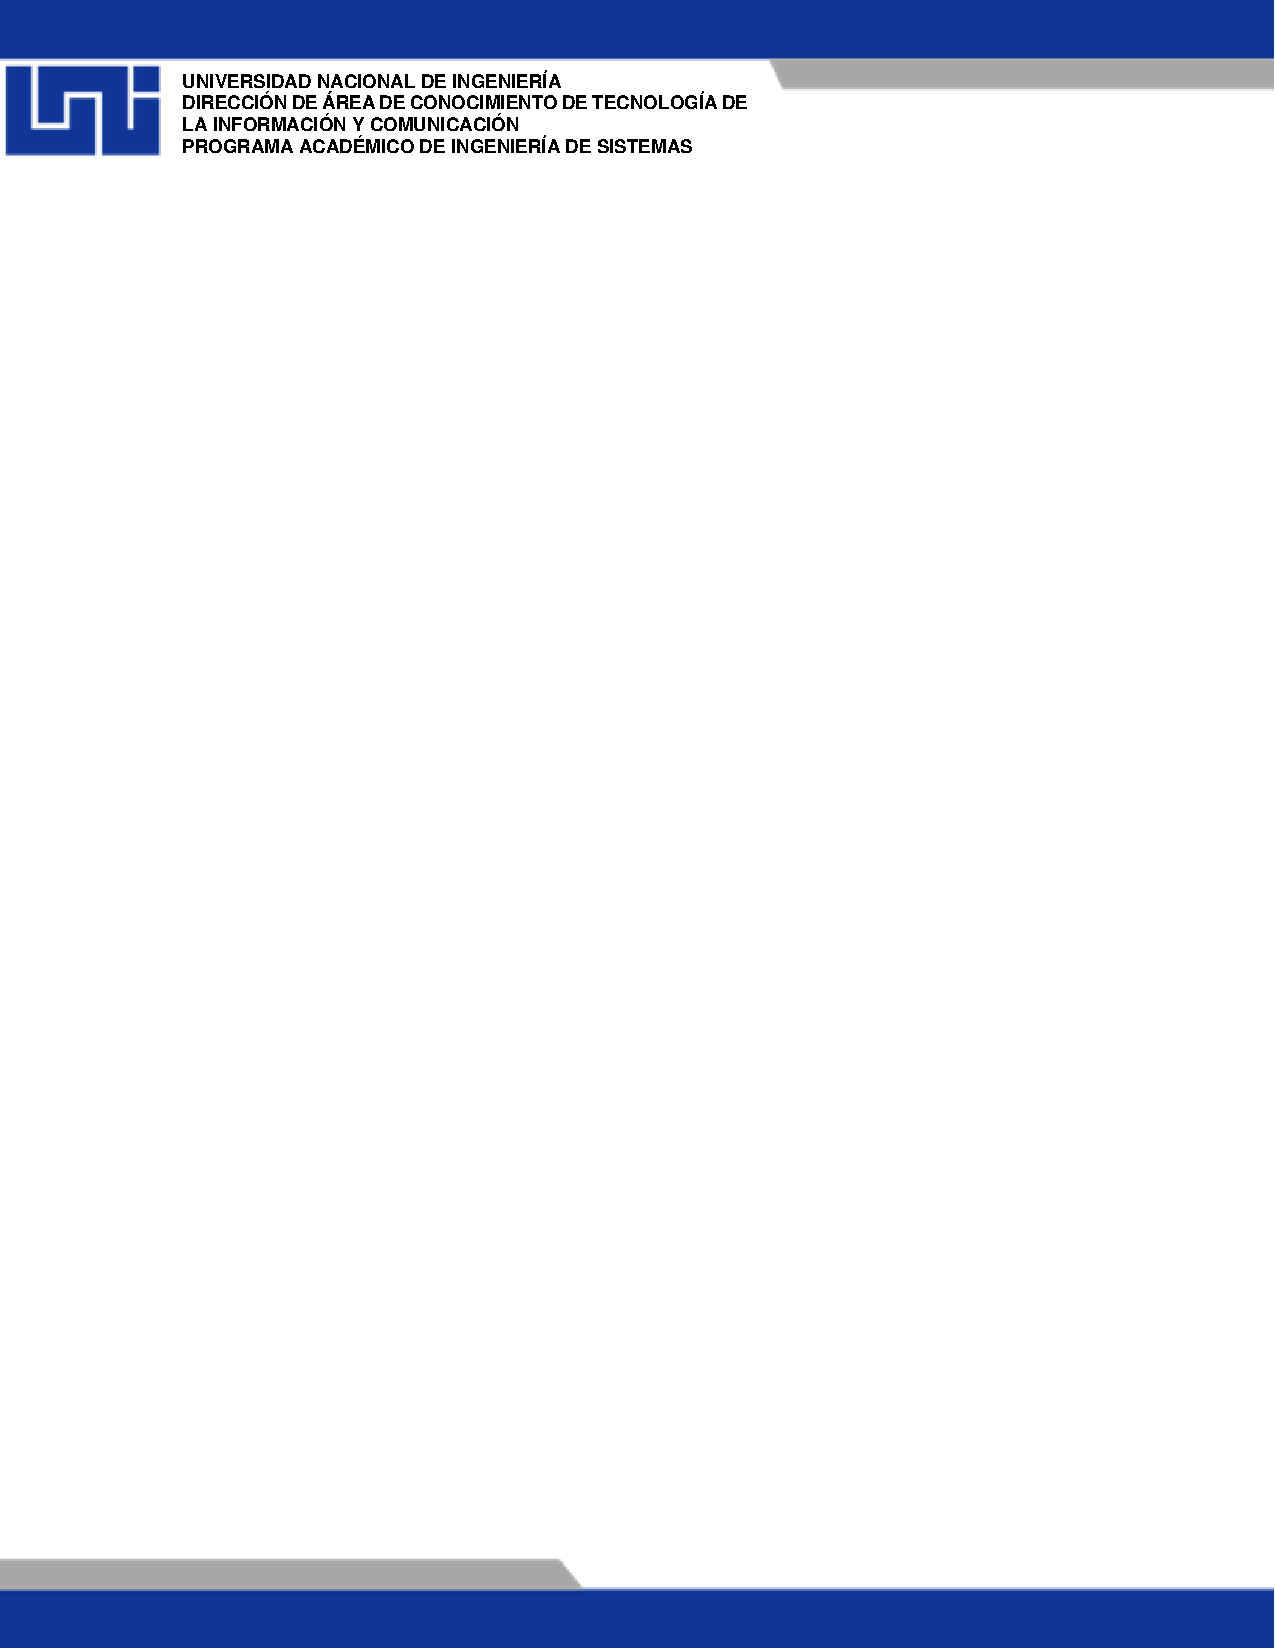
\includegraphics[width=\paperwidth,height=\paperheight]{fondo.pdf}%
    }%
  }%
}
% --------------------------------------------------

\begin{document}
\FondoPortada % Esto activa el fondo solo para esta página
\printanswers
\shadedsolutions
\thispagestyle{empty}
\renewcommand{\solutiontitle}{\noindent\textbf{Solución:} }
\renewcommand{\thepartno}{\arabic{partno}}

\begin{center}
{\textbf{Segundo Sistemático}}
\end{center}
\begin{minipage}[t]{.6\textwidth}%
  {\bfseries Nombres}: \makebox[.75\textwidth]{\hrulefill} \par
  \vspace{1ex}
  {\bfseries Apellidos}: \makebox[.75\textwidth]{\hrulefill} \par
  \vspace{1ex}
    {\bfseries Docente}: Ricardo Largaespada \par
  \vspace{1ex}
\end{minipage}%
\hfill
\begin{minipage}[t]{.4\textwidth}%
  {\bfseries Curso}: Matemática I\par
  \vspace{1ex}
  {\bfseries Fecha}: 27 de marzo 2026 \par
  \vspace{1ex}
  {\bfseries Grupo}: 1M6-SIS\par
  \vspace{1ex}
\end{minipage}%
\begin{center}
  \rule{\textwidth}{1pt}
\end{center}

\noindent\underline{\sc Instrucciones a estudiantes}
\begin{enumerate}
\item Este sistemático contiene {\bf SESENTA (60)} preguntas, las cuales debes resolver en grupos de 5 personas.
\item Puedes utilizar calculadora. Sin embargo, debes escribir los pasos del trabajo.
\item Entrega todo el trabajo adicional en páginas rotuladas.
\end{enumerate}

\rule[1ex]{\textwidth}{1pt}

\qformat{Pregunta \thequestion: \thequestiontitle\dotfill\thepoints}
\pointname{\%}

\begin{questions}
\titledquestion{Asíntotas de Funciones}[20]
Hallar las asíntotas de las siguientes funciones.
\begin{multicols}{2}
\begin{parts}
\part $y(x-3)^2=x^2+9$ \begin{solution} $x=3$ y $y=1$ \end{solution}
\part $x^2(x+y)=a^2(x-y)$ \begin{solution} $y=-x$ \end{solution}
\part $xy^2-3y^2-4x=8$ \begin{solution} $x=3$, $y=-2$ y $y=2$ \end{solution}
\part $y=\sqrt{x^2+x}-x$ \begin{solution} $y=\frac{1}{2}$ \end{solution}
\part $xy^2+yx^2=a^3$ \begin{solution} $x=0$, $y=0$ y $y=-x$ \end{solution}
\part $y=\frac{x^2+3}{\sqrt{x^2+1}}$ \begin{solution} $y=-x$ y $y=x$ \end{solution}
\part $y=\frac{x^2+2x-1}{x}$ \begin{solution} $x=0$ y $y=\pm x$ \end{solution}
\part $y=3-2x-\frac{x^2}{\sqrt{x^2-x-2}}$ \begin{solution} $x=1$, $y=2$, $y=-3x+\frac{5}{2}$, $y=-x-\frac{7}{2}$ \end{solution}
\part $y=\frac{\sqrt{1-x^2}}{x^2-4}$ \begin{solution} $y=-1$ y $x=\pm 2$ \end{solution}
\part $y=\frac{x-5}{x^2-7x+10}$ \begin{solution} $x=5$ y $x=2$ \end{solution}
\end{parts}
\end{multicols}

\titledquestion{Límites Trigonométricos}[40]
Resuelve los siguientes límites:
\begin{multicols}{2}
\begin{parts}
\part $\displaystyle \lim_{x\to\pi} \frac{1-\sin \frac{x}{2}}{\pi-x}$ \begin{solution} $0$ \end{solution}
\part $\displaystyle \lim_{x\to 0} \frac{\cos x -\cos 3x}{x^2}$ \begin{solution} $4$ \end{solution}
\part $\displaystyle \lim_{x\to 0}  \frac{\tan x-\sin x}{x^3}$ \begin{solution} $\frac{1}{2}$ \end{solution}
\part $\displaystyle \lim_{x\to 0}\frac{x-\sin 2x}{x+\sin 3x}$ \begin{solution} $-\frac{1}{4}$ \end{solution}
\part $\displaystyle \lim_{x\to 0} \frac{1-\sqrt{\cos x}}{x^2}$ \begin{solution} $\frac{1}{4}$ \end{solution}
\part $\displaystyle \lim_{x\to 0} \frac{1-\cos^7 x}{x^2}$ \begin{solution} $\frac{7}{2}$ \end{solution}
\part $\displaystyle \lim_{x\to\frac{\pi}{2}} \frac{1-\sin x}{(\pi/2-x)^2}$ \begin{solution} $\frac{1}{2}$ \end{solution}
\part $\displaystyle \lim_{x\to \frac{\pi}{4}}\frac{\cos x-\sin x}{\cos 2x}$ \begin{solution} $\frac{\sqrt{2}}{2}$ \end{solution}
\part $\displaystyle \lim_{x\to 1}(1-x)\tan \frac{\pi x}{2}$ \begin{solution} $\frac{2}{\pi}$ \end{solution}
\part $\displaystyle \lim_{x\to 1} \frac{\cos\left(\frac{\pi x}{2}\right)}{1-\sqrt{x}}$ \begin{solution} $\pi$ \end{solution}
\part $\displaystyle \lim_{x\to \frac{2\pi}{3}} \frac{\sin 6x}{3x-2\pi}$ \begin{solution} $2$ \end{solution}
\part $\displaystyle \lim_{h\to 0}\frac{\sin^2(h+a)-\sin^2 a}{h}$ \begin{solution} $\sin 2a$ \end{solution}
\part $\displaystyle \lim_{x\to 0}\frac{\sin 3x\cdot \sin 5x}{(x-x^3)^2}$ \begin{solution} $15$ \end{solution}
\part $\displaystyle \lim_{x\to 0}\frac{3\sin\pi x-\sin 3\pi x}{x^3}$ \begin{solution} $4\pi^3$ \end{solution}
\part $\displaystyle \lim_{x\to 0} \frac{\sqrt{x^2+4}-3\cos x+1}{1-\cos x}$ \begin{solution} $\frac{7}{2}$ \end{solution}
\part $\displaystyle \lim_{x\to 0} \frac{\tan(a+2x)-2\tan(a+x)+\tan a}{x^2}$ \begin{solution} $\frac{2\sin a}{\cos^3 a}$ \end{solution}
\part $\displaystyle \lim_{x\to 0}\frac{(1-\cos x)^2}{\tan^3 x-\sin^3 x}$ \begin{solution} $\infty$ \end{solution}
\part $\displaystyle \lim_{x\to \frac{\pi}{2}}\frac{\cos x}{\frac{\pi}{2}-x}$ \begin{solution} $1$ \end{solution}
\part $\displaystyle \lim_{x\to 0} \frac{\tan ax-\tan^3 ax}{\tan x}$ \begin{solution} $a$ \end{solution}
\part $\displaystyle \lim_{x\to \frac{\pi}{2}} \frac{(1-\sin x)^3}{(1+\cos 2x)^3}$ \begin{solution} $\frac{1}{64}$ \end{solution}
\part $\displaystyle \lim_{x\to 0} \frac{\tan ax}{(1-\cos ax+x)\sec ax}$ \begin{solution} $a$ \end{solution}
\part $\displaystyle \lim_{x\to 5} \frac{\sin(x^2-10x+25)}{x^3+5x^2-125x+375}$ \begin{solution} $\frac{1}{20}$ \end{solution}
\part $\displaystyle \lim_{x\to 0} \left(\frac{2}{\sin^2 x}-\frac{1}{1-\cos x}\right)$ \begin{solution} $\frac{1}{2}$ \end{solution}
\part $\displaystyle \lim_{x\to 0} \frac{x\sin(\sin 2x)}{1-\cos(\sin 4x)}$ \begin{solution} $\frac{1}{4}$ \end{solution}
\part $\displaystyle \lim_{x\to \frac{\pi}{2}} \frac{\cos x}{\sqrt{1-\sin x}}$ \begin{solution} $\sqrt{2}$ \end{solution}
\end{parts}
\end{multicols}


\titledquestion{Límites Exponenciales y Logarítmicos}[40]
\begin{multicols}{2}
\begin{parts}
\part $\displaystyle \lim_{x\to\infty}\left( \frac{x^3+2x+3}{x^3+4}\right)^{x^2+2}$ \begin{solution} $e^2$ \end{solution}
\part $\displaystyle \lim_{x\to\infty}\left( \frac{x^2-2x+1}{x^2-4x+2}\right)^{x}$ \begin{solution} $e^2$ \end{solution}
\part $\displaystyle \lim_{x\to\infty}\left( \frac{3x-4}{3x+2}\right)^{\frac{x+1}{3}}$ \begin{solution} $e^{-2/3}$ \end{solution}
\part $\displaystyle \lim_{x\to 0}\left( \cos x+\sin x\right)^{\frac{1}{x}}$ \begin{solution} $e$ \end{solution}
\part $\displaystyle \lim_{x\to 0} \frac{\ln{a+x}-\ln{a}}{x}$ \begin{solution} $\frac{1}{a}$ \end{solution}
\part $\displaystyle \lim_{x\to\infty}\left( \frac{x+a}{x-a}\right)^{x}$ \begin{solution} $e^{2a}$ \end{solution}
\part $\displaystyle \lim_{x\to\infty}\left( \frac{x^3+2x+3}{x^3+4}\right)^{\frac{1-x^3}{x}}$ \begin{solution} $e^{-2}$ \end{solution}
\part $\displaystyle \lim_{x\to 0}\left( 1-\sin 3x\right)^{\frac{1}{2x}}$ \begin{solution} $e^{-3/2}$ \end{solution}
\part $\displaystyle \lim_{x\to 0}\left( e^x+ x\right)^{\frac{m}{x}}$ \begin{solution} $e^{2m}$ \end{solution}
\part $\displaystyle \lim_{x\to 0} \left( x+e^x \right)^{\frac{1}{x}}$ \begin{solution} $e^2$ \end{solution}
\part $\displaystyle \lim_{x\to 0}\left( \frac{1+\tan x}{1-\sin x}\right)^{\frac{1}{\sin x}}$ \begin{solution} $e^2$ \end{solution}
\part $\displaystyle \lim_{x\to 0}\sqrt{2-\sqrt{\cos x}}^{\frac{1}{x^2}}$ \begin{solution} $1$ \end{solution}
\part $\displaystyle \lim_{x\to 0}\left( \cos x \right)^{\frac{1}{x^2}}$ \begin{solution} $e^{-1/2}$ \end{solution}
\part $\displaystyle \lim_{x\to \infty}\left( \cos\sqrt{\frac{5a}{x}}\right)^{bx}$ \begin{solution} $e^{-\frac{15ab}{2}}$ \end{solution}
\part $\displaystyle \lim_{x\to 0} \left(\frac{(e^x+x)^{\tan x}}{(1+\sin x)^x}\right)^{\frac{\cot x}{x}}$ \begin{solution} $\frac{1}{a}$ \end{solution}
\part $\displaystyle \lim_{x\to 0} \frac{\ln(\cos x)}{x^2}$ \begin{solution} $-\frac{1}{2}$ \end{solution}
\part $\displaystyle \lim_{x\to 0}\left(\frac{\sin x}{x}\right)^{\frac{\sin x}{x-\sin x}}$ \begin{solution} $\frac{1}{e}$ \end{solution}
\part $\displaystyle \lim_{x\to 0}\frac{\ln(\cos ax)}{\ln(\cos bx)}$ \begin{solution} $ \left(\frac{a}{b}\right)^2$ \end{solution}
\part $\displaystyle \lim_{x\to -\infty} \frac{\ln(1+e^x)}{x}$ \begin{solution} $0$ \end{solution}
\part $\displaystyle \lim_{x\to +\infty} \frac{\ln(1+e^x)}{x}$ \begin{solution} $1$ \end{solution}
\part $\displaystyle \lim_{x\to a} \frac{x-a}{\ln x-\ln a}$ \begin{solution} $a$ \end{solution}
\part $\displaystyle \lim_{x\to 0} \frac{e^{ax}-1}{e^{bx}-1}$ \begin{solution} $ \frac{a}{b}$ \end{solution}
\part $\displaystyle \lim_{x\to b} \frac{a^x-a^b}{x-b},a>0$ \begin{solution} $a^b\ln a$ \end{solution}
\part $\displaystyle \lim_{x\to 0} \frac{1}{ax}\ln \sqrt[3]{\frac{1+ax}{1-ax}}$ \begin{solution} $ \frac{2}{3}$ \end{solution}
\part $\displaystyle \lim_{x\to 0} \frac{5^x-4^x}{x^2-x}$ \begin{solution} $ -\ln\frac{5}{4}$ \end{solution}
\end{parts}
\end{multicols}
\end{questions}

\end{document}